The convolutional multilayer kernel is a generalization of the hierarchical kernel
descriptors introduced in computer vision~\cite{bo2011,bo2010}. The kernel produces a
sequence of image representations that are built on top of each other in a
multilayer fashion. Each layer can be interpreted as a non-linear
transformation of the previous one with additional spatial invariance. We call these
layers \emph{image feature maps}\footnote{In the kernel literature, ``feature map'' denotes the mapping between data points and their representation in a reproducing kernel Hilbert space (RKHS)~\cite{shawe2004}. Here, feature maps refer to spatial maps representing local image characteristics at everly location, as usual in the neural network literature~\cite{lecun1998}.}, and formally define them as follows:
\begin{definition}
   An image feature map~ is a function~, where~ is a (usually discrete) subset of~
   representing normalized ``coordinates'' in the image and~ is a Hilbert space.
\end{definition}
For all practical examples in this paper,  is a two-dimensional grid
and corresponds to different locations in a two-dimensional image. In other
words,  is a set of pixel coordinates. Given~ in~, the
point~ represents some characteristics of the image at
location~, or in a neighborhood of~.
For instance, a color image of size~ with three
channels, red, green, and blue, may be represented by an initial feature
map~, where~ is an~ regular grid,  is the Euclidean space , and 
provides the color pixel values. With the multilayer scheme, non-trivial feature maps will be
obtained subsequently, which will encode more complex image characteristics.
With this terminology in hand, we now introduce the convolutional kernel, first, for a single layer.

\begin{definition}[\bfseries Convolutional Kernel with Single Layer] \label{def:scattering}
   Let us consider two images represented by two
   image feature maps, respectively~ and~,
   where~ is a set of pixel locations, and~ is a Hilbert space.
   The one-layer convolutional kernel between~ and~ is defined as 
  
  where~ and~ are smoothing parameters of Gaussian kernels,
  and~ if~ and~ otherwise.
  Similarly,  is a normalized version of~.\footnote{When~ is not discrete, the notation~ in~(\ref{eq:kernel}) should be replaced by the Lebesgue integral~ in the paper.}
\end{definition}
\vspace*{-0.1cm}
It is easy to show that the kernel~ is positive definite (see Appendix~A). It consists of a sum of pairwise
comparisons between the image features~ and~ computed at
all spatial locations~ and~ in~. To be significant in the sum, a
comparison needs the corresponding  and~ to be close 
in~, and the normalized features  and
 to be close in the feature space~. 
The parameters~ and~ respectively control these two definitions
of ``closeness''. Indeed, when~
is large, the kernel~ is invariant to the positions~ and~ but
when~ is small, only features placed at the same location  are
compared to each other. Therefore, the role of~ is to control how much the kernel
is locally shift-invariant. Next, we will show how to go beyond one single
layer, but before that, we present concrete examples of simple input
feature maps~.
\vs
\paragraph{Gradient map.} Assume that  and that
 provides the two-dimensional gradient of the image at
pixel~, which is often computed with first-order differences along each
dimension. Then, the quantity  is the gradient intensity, and~ is its orientation,
which can be characterized by a particular angle---that is, there exists~
in~ such that . The
resulting kernel~ is exactly the kernel descriptor introduced in
\cite{bo2011,bo2010} for natural image patches.

\vs
\paragraph{Patch map.} In that setting,  associates to a
location~ an image patch of size~ centered at~.
Then, the space~ is simply~, and~ is a \emph{contrast-normalized}
version of the patch, which is a useful transformation for visual recognition according
to classical findings in computer vision~\cite{jarrett2009}. When the
image is encoded with three color channels, patches are of size~.

We now define the multilayer convolutional kernel,
generalizing some ideas of~\cite{bo2011}.

\begin{definition}[\bfseries Multilayer Convolutional Kernel]\label{def:multiscattering}
   Let us consider a set  and a Hilbert space .
   We build a new set~ and a new Hilbert space~ as follows:

   (i) choose a patch shape~ defined as a bounded symmetric subset
   of~, and a set of coordinates~
   such that for all location~ in~, the patch~ is a subset of~;\footnote{For two sets~
   and~, the Minkowski sum  is defined as .\label{foot:minkowski}}
   In other words, each coordinate~ in~ corresponds to a valid patch in~ centered at~.

   (ii) define the convolutional kernel~ on the ``patch'' feature maps~, by replacing in~(\ref{eq:kernel}):~ by~,~
   by~, and~ by appropriate smoothing
   parameters~. We denote by~ the Hilbert space for
   which the positive definite kernel~ is reproducing.

   An image represented by a feature map~ at layer~ is now encoded in the~-th layer as~, where for all~ in~,~ is the representation
   in~ of the patch feature map~ for~ in~.
\end{definition}
Concretely, the kernel~ between two patches of~ and~ at respective locations~ and~~is
\vspace*{-0.1cm}

where~ is the Hilbertian norm of~.
In Figure~\ref{subfig:hierarchy}, we illustrate the interactions
between the sets of coordinates~, patches~, and feature spaces~ across
layers. For two-dimensional grids, a typical patch
shape is a square, for example~ for a  patch in an image of size~. Information encoded in the~-th layer differs from the~-th one in two aspects:
first, each point~ in layer~ contains
information about several points from the -th layer and can possibly represent
larger patterns; second, the new feature map is more locally shift-invariant than the previous one due to the
term involving the parameter~ in~(\ref{eq:kernelpatch}). 

\pgfdeclarelayer{bottom}  \pgfdeclarelayer{middle}\pgfdeclarelayer{top}
\pgfsetlayers{bottom,middle,top}  
\begin{figure}
   \subfigure[Hierarchy of image feature maps.]{\label{subfig:hierarchy}
      \hspace*{-0.4cm}
   \begin{tikzpicture}[scale=1,every node/.style={minimum size=1cm},on grid]
      \begin{pgfonlayer}{bottom}
         \begin{scope}[  yshift=0,every node/.append style={
               yslant=0.5,xslant=-1,rotate=-10},yslant=0.5,xslant=-1,rotate=-10
            ]
            \fill[white,fill opacity=0.9] (0,0) rectangle (3,3);
            \draw[step=2mm, gray!70] (0,0) grid (3,3);
            \draw[black] (0,0) rectangle (3,3);
            \draw[red!20,fill] (0.4,0.6) rectangle (0.6,0.8);
            \draw[red!80!black!100] (0.4,0.6) rectangle (0.6,0.8);
            \draw[blue!20,fill] (1,0.4) rectangle (1.8,1.2);
            \draw[blue!90] (1,0.4) rectangle (1.8,1.2);
            \draw[step=2mm, blue!70] (1,0.4) grid (1.8,1.2);
            \coordinate (a) at (0.5,0.7);
            \coordinate (B1) at (1,0.4);
            \coordinate (B2) at (1,1.2);
            \coordinate (B3) at (1.8,0.4);
            \coordinate (B4) at (1.8,1.2);
            \coordinate (B5) at (1.4,0.8);
            \coordinate (aa) at (1,0);
         \end{scope}
         \draw[-latex,thick] (1.8,0.1) node[right]{}to[out=180,in=-50] (aa);
         \draw[-latex,thick] (-0.3,0) node[left]{{\color{red!80!black!80} }}to[out=0,in=270] (a);
         \draw[-latex,thick] (2.2,0.5) node[right]{{\color{blue!80!black!80} }}to[out=180,in=50] (B5);
      \end{pgfonlayer}
      \begin{pgfonlayer}{middle}
         \begin{scope}[  
               yshift=50,every node/.append style={
               yslant=0.5,xslant=-1,rotate=-10},yslant=0.5,xslant=-1,rotate=-10
            ]
            \fill[white,fill opacity=.7] (0,0) rectangle (2.1,2.1);
            \draw[green!20,fill] (0,0.9) rectangle (0.9,1.8);
            \draw[step=3mm, gray!70] (0,0) grid (2.1,2.1);
            \draw[black] (0,0) rectangle (2.1,2.1);
            \draw[blue!20,fill] (0.9,0.3) rectangle (1.2,0.6);
            \draw[blue!90] (0.9,0.3) rectangle (1.2,0.6);
            \draw[green!70!black!100] (0,0.9) rectangle (0.9,1.8);
            \draw[step=3mm, green!70] (0,0.9) grid (0.9,1.8);
            \coordinate (b) at (1.05,0.45);
            \coordinate (c) at (0,1.5);
            \coordinate (A1) at (0.9,0.3);
            \coordinate (A2) at (0.9,0.6);
            \coordinate (A3) at (1.2,0.3);
            \coordinate (A4) at (1.2,0.6);
            \coordinate (D1) at (0,0.9);
            \coordinate (D2) at (0,1.8);
            \coordinate (D3) at (0.9,0.9);
            \coordinate (D4) at (0.9,1.8);
            \coordinate (D5) at (0.45,1.35);
         \end{scope}
      \draw[-latex,thick] (2.2,2.3) node[right]{{\color{blue!80!black!80}}}to[out=180,in=50] (b);
      \draw[-latex,thick] (-1.8,2.4) node[left]{}to[out=0,in=180] (c);
      \draw[-latex,thick] (2.2,3.5) node[right]{{\color{green!60!black!100} }}to[out=180,in=50] (D5);
      \end{pgfonlayer}
      \begin{pgfonlayer}{bottom}
         \draw[thick,blue!70] (A1) -- (B1);
         \draw[thick,blue!70] (A2) -- (B2);
         \draw[thick,blue!70] (A3) -- (B3);
         \draw[thick,blue!70] (A4) -- (B4);
      \end{pgfonlayer}
      \begin{pgfonlayer}{top}
         \begin{scope}[  yshift=100,every node/.append style={
               yslant=0.5,xslant=-1,rotate=-10},yslant=0.5,xslant=-1,rotate=-10
            ]
            \fill[white,fill opacity=.7] (0,0) rectangle (1.6,1.6);
            \draw[step=4mm, gray!70] (0,0) grid (1.6,1.6);
            \draw[black] (0,0) rectangle (1.6,1.6);
            \draw[green!20,fill] (0,0.8) rectangle (0.4,1.2);
            \draw[green!70!black!100] (0,0.8) rectangle (0.4,1.2);
            \coordinate (CC1) at (0,1.6);
            \coordinate (CC2) at (0.2,1.0);
            \coordinate (C1) at (0,0.8);
            \coordinate (C2) at (0,1.2);
            \coordinate (C3) at (0.4,0.8);
            \coordinate (C4) at (0.4,1.2);
         \end{scope}
         \draw[-latex,thick] (-1.8,4.2) node[left]{}to[out=0,in=180] (CC1);
         \draw[-latex,thick] (2.2,4.8) node[right]{{\color{green!60!black!100}}}to[out=180,in=50] (CC2);
      \end{pgfonlayer}
      \begin{pgfonlayer}{middle}
         \draw[thick,green!70!black!100] (C1) -- (D1);
         \draw[thick,green!70!black!100] (C2) -- (D2);
         \draw[thick,green!70!black!100] (C3) -- (D3);
         \draw[thick,green!70!black!100] (C4) -- (D4);
      \end{pgfonlayer}
   \end{tikzpicture}
   }
   \subfigure[Zoom between layer~ and~ of the CKN.]{\label{subfig:convnet}
      \hspace*{-0.3cm}
      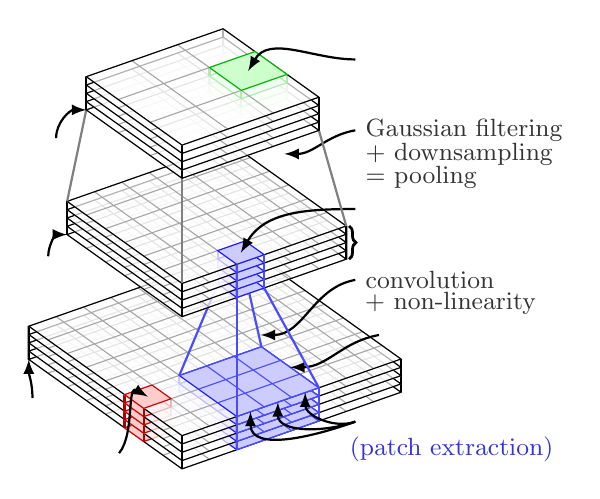
\begin{tikzpicture}[decoration={brace}][scale=1,every node/.style={minimum size=1cm},on grid]
         \begin{pgfonlayer}{bottom}
            \newcount\mycount
            \foreach \i in {0,1,2,3,4} {
               \mycount=\i
               \multiply\mycount by 3
               \begin{scope}[  yshift=\mycount,every node/.append style={
                     yslant=0.5,xslant=-1,rotate=-10},yslant=0.5,xslant=-1,rotate=-10
                  ]
                  \coordinate (X\i) at (0.15,0.75);
                  \coordinate (G\i) at (1.5,0.45);
                  \coordinate (ZA\i) at (1.05,0);
                  \coordinate (ZB\i) at (1.35,0);
                  \coordinate (ZC\i) at (0.75,0);
                  \coordinate (AAA\i) at (0,0);
                  \coordinate (AAB\i) at (0,2.4);
                  \coordinate (AAC\i) at (2.4,0);
                  \coordinate (AAD\i) at (2.4,2.4);
                  \coordinate (AA\i) at (0.6,0);
                  \coordinate (AB\i) at (0.6,0.9);
                  \coordinate (AC\i) at (1.5,0);
                  \coordinate (AD\i) at (1.5,0.9);
                  \coordinate (EA\i) at (0,0.6);
                  \coordinate (EB\i) at (0,0.9);
                  \coordinate (EC\i) at (0.3,0.6);
                  \coordinate (ED\i) at (0.3,0.9);
                  \newcount\prevcount
                  \prevcount=\i
                  \advance\prevcount by -1
                  \ifnum\i>0
                  \draw[thick,blue!70] (AA\i) -- (AA\the\prevcount);
                  \draw[thick,blue!70] (AB\i) -- (AB\the\prevcount);
                  \draw[thick,blue!70] (AC\i) -- (AC\the\prevcount);
                  \draw[thick,blue!70] (AD\i) -- (AD\the\prevcount);
                  \draw[thick,red!70!black!100] (EA\i) -- (EA\the\prevcount);
                  \draw[thick,red!70!black!100] (EB\i) -- (EB\the\prevcount);
                  \draw[thick,red!70!black!100] (EC\i) -- (EC\the\prevcount);
                  \draw[thick,red!70!black!100] (ED\i) -- (ED\the\prevcount);
                  \draw[thick,black] (AAA\i) -- (AAA\the\prevcount);
                  \draw[thick,black] (AAB\i) -- (AAB\the\prevcount);
                  \draw[thick,black] (AAC\i) -- (AAC\the\prevcount);
                  \draw[thick,black] (AAD\i) -- (AAD\the\prevcount);
                  \fi
                  \fill[white,fill,opacity=.7] (0,0) rectangle (2.4,2.4);
                  \draw[step=3mm, gray!70] (0,0) grid (2.4,2.4);
                  \draw[black] (0,0) rectangle (2.4,2.4);
                  \draw[blue!20,fill] (0.6,0) rectangle (1.5,0.9);
                  \draw[blue!90] (0.6,0) rectangle (1.5,0.9);
                  \draw[step=3mm, blue!70] (0.6,0) grid (1.5,0.9);
                  \draw[red!20,fill] (0,0.6) rectangle (0.3,0.9);
                  \draw[red!80!black!100] (0,0.6) rectangle (0.3,0.9);
               \end{scope}
            }
            \draw[-latex,thick] (-1.9,0.9) node[below,xshift=1mm,yshift=2mm]{{\color{black} }}to[out=90,in=270] (AAB0);
            \draw[-latex,thick] (-0.8,0.2) node[left]{{\color{red!80!black!80} }}to[out=50,in=150] (X4);
            \draw[-latex,thick] (2.2,0.6) node[right]{{\color{blue!80!black!80} }}to[out=200,in=-90] (ZA4);
            \draw[-latex,thick,white] (2,0.25) node[right]{{\color{blue!80!black!80}\small (patch extraction)}}to[out=200,in=-90] (2.2,0.5);
            \draw[-latex,thick] (2.2,0.6) node[right]{}to[out=200,in=-90] (ZB4);
            \draw[-latex,thick] (2.2,0.6) node[right]{}to[out=200,in=-90] (ZC4);
            \draw[-latex,thick] (2.5,1.7) node[right]{{\color{blue!80!black!80}  }}to[out=190,in=0] (G4);
            \draw[-latex,thick] (2.2,2.4) node[right]{{\color{black!80} \small convolution}}to[out=190,in=0] (1.0,1.7);
            \draw[-latex,white] (2.2,2.1) node[right]{{\color{black!80} \small + non-linearity}}to[out=150,in=-90] (2.2,2.1);
         \end{pgfonlayer}
         \begin{pgfonlayer}{middle}
            \newcount\mycount
            \foreach \i in {0,1,2,3,4} {
               \mycount=\i
               \multiply\mycount by 3
               \advance\mycount by 55
               \begin{scope}[  
                     yshift=\mycount,every node/.append style={
                     yslant=0.5,xslant=-1,rotate=-10},yslant=0.5,xslant=-1,rotate=-10
                  ]
                  \coordinate (W\i) at (0.75,0.15);
                  \coordinate (BAA\i) at (0,0);
                  \coordinate (BAB\i) at (0,1.8);
                  \coordinate (BAC\i) at (1.8,0);
                  \coordinate (BAD\i) at (1.8,1.8);
                  \coordinate (BA\i) at (0.6,0);
                  \coordinate (BB\i) at (0.6,0.3);
                  \coordinate (BC\i) at (0.9,0);
                  \coordinate (BD\i) at (0.9,0.3);
                  \newcount\prevcount
                  \prevcount=\i
                  \advance\prevcount by -1
                  \ifnum\i>0
                  \draw[thick,blue!70] (BA\i) -- (BA\the\prevcount);
                  \draw[thick,blue!70] (BB\i) -- (BB\the\prevcount);
                  \draw[thick,blue!70] (BC\i) -- (BC\the\prevcount);
                  \draw[thick,blue!70] (BD\i) -- (BD\the\prevcount);
                  \draw[thick,black] (BAA\i) -- (BAA\the\prevcount);
                  \draw[thick,black] (BAB\i) -- (BAB\the\prevcount);
                  \draw[thick,black] (BAC\i) -- (BAC\the\prevcount);
                  \draw[thick,black] (BAD\i) -- (BAD\the\prevcount);
                  \fi
                  \fill[white,fill,opacity=.7] (0,0) rectangle (1.8,1.8);
                  \draw[step=3mm, gray!70] (0,0) grid (1.8,1.8);
                  \draw[black] (0,0) rectangle (1.8,1.8);
                  \draw[blue!20,fill] (0.6,0) rectangle (0.9,0.3);
                  \draw[blue!90] (0.6,0) rectangle (0.9,0.3);
               \end{scope}
            }
            \draw[decorate,decoration={brace,mirror,raise=1pt},line width=1pt] (BAC0) -- (BAC4) node[right,yshift=-2mm,xshift=1mm] {};
            \draw[-latex,thick] (2.2,3.3) node[right]{{\color{blue!80!black!80} }}to[out=180,in=60] (W4);
            \draw[-latex,thick] (-1.7,2.7) node[below,yshift=3mm]{{\color{black} }}to[out=90,in=180] (BAB0);
            \draw[-latex,thick] (2.2,4.3) node[right]{{\color{black!80} \small Gaussian filtering}}to[out=190,in=0] (1.3,4);
            \draw[-latex,thick,white] (2.2,4) node[right]{{\color{black!80} \small + downsampling}}to[out=190,in=0] (2.2,4);
            \draw[-latex,thick,white] (2.2,3.7) node[right]{{\color{black!80} \small = pooling}}to[out=190,in=0] (2.2,3.7);
         \end{pgfonlayer}
         \begin{pgfonlayer}{bottom}
            \draw[thick,blue!70] (BA0) -- (AA4);
            \draw[thick,blue!70] (BB0) -- (AB4);
            \draw[thick,blue!70] (BC0) -- (AC4);
            \draw[thick,blue!70] (BD0) -- (AD4);
         \end{pgfonlayer}
         \begin{pgfonlayer}{top}
            \foreach \i in {0,1,2,3,4} {
               \mycount=\i
               \multiply\mycount by 3
               \advance\mycount by 105
               \begin{scope}[  yshift=\mycount,every node/.append style={
                     yslant=0.5,xslant=-1,rotate=-10},yslant=0.5,xslant=-1,rotate=-10
                  ]
                  \coordinate (H\i) at (1.25,0.75);
                  \coordinate (CAA\i) at (0,0);
                  \coordinate (CAB\i) at (0,1.5);
                  \coordinate (CAC\i) at (1.5,0);
                  \coordinate (CAD\i) at (1.5,1.5);
                  \coordinate (CA\i) at (1.0,0.5);
                  \coordinate (CB\i) at (1.0,1.0);
                  \coordinate (CC\i) at (1.5,0.5);
                  \coordinate (CD\i) at (1.5,1.0);
                  \newcount\prevcount
                  \prevcount=\i
                  \advance\prevcount by -1
                  \ifnum\i>0
                  \draw[thick,black] (CAA\i) -- (CAA\the\prevcount);
                  \draw[thick,black] (CAB\i) -- (CAB\the\prevcount);
                  \draw[thick,black] (CAC\i) -- (CAC\the\prevcount);
                  \draw[thick,black] (CAD\i) -- (CAD\the\prevcount);
                  \draw[thick,green!70!black!100] (CA\i) -- (CA\the\prevcount);
                  \draw[thick,green!70!black!100] (CB\i) -- (CB\the\prevcount);
                  \draw[thick,green!70!black!100] (CC\i) -- (CC\the\prevcount);
                  \draw[thick,green!70!black!100] (CD\i) -- (CD\the\prevcount);
                  \fi
                  \fill[white,fill,opacity=.7] (0,0) rectangle (1.5,1.5);
                  \draw[step=5mm, gray!70] (0,0) grid (1.5,1.5);
                  \draw[black] (0,0) rectangle (1.5,1.5);
                  \draw[green!20,fill] (1.0,0.5) rectangle (1.5,1.0);
                  \draw[green!70!black!100] (1.0,0.5) rectangle (1.5,1.0);
               \end{scope}
            }
            \draw[-latex,thick] (-1.6,4.2) node[below,yshift=3mm]{{\color{black} }}to[out=90,in=180] (CAB0);
            \draw[-latex,thick] (2.2,5.2) node[right]{{\color{green!60!black!100} }}to[out=180,in=60] (H4);
         \end{pgfonlayer}
         \begin{pgfonlayer}{middle}
            \draw[thick,black!50] (CAA0) -- (BAA4);
            \draw[thick,black!50] (CAB0) -- (BAB4);
            \draw[thick,black!50] (CAC0) -- (BAC4);
            \draw[thick,black!50] (CAD0) -- (BAD4);
         \end{pgfonlayer}
      \end{tikzpicture}
      \label{subfig:cnn}
   }
   \vspace*{-0.3cm}
   \caption{Left: concrete representation of the successive layers for the multilayer convolutional kernel. Right: one layer of the convolutional neural network that approximates the kernel.
   }\label{fig:sketch}
\end{figure}

The multilayer convolutional kernel slightly differs from the hierarchical kernel descriptors
of~\cite{bo2011} but exploits similar ideas. Bo et al.~\cite{bo2011} define
indeed several ad hoc kernels for representing local information in images,
such as gradient, color, or shape. These kernels are close to the one
defined in~(\ref{eq:kernel}) but with a few variations. Some of them do not
use normalized features~, and these kernels use different
weighting strategies for the summands of~(\ref{eq:kernel}) that are specialized
to the image modality, \eg, color, or gradient, whereas we use the same
weight~ for all kernels. The generic
formulation~(\ref{eq:kernel}) that we propose may be useful per
se, but our main contribution comes in the next section, where we use the  
kernel as a new tool for learning convolutional neural networks.

